\documentclass[12pt]{article}

\usepackage{subfigure}
\usepackage{booktabs}

%\pagestyle{plain}
%\pagenumbering{arabic}
\usepackage{amsmath,amsfonts,epsfig,amssymb}
\usepackage{amsthm}

\usepackage{graphics}
\usepackage{graphicx}
\usepackage{chemarrow}
\usepackage{extarrows}
\usepackage{subfigure}
\usepackage{dsfont}
\usepackage{multirow}
\usepackage{latexsym}
\usepackage{float}
\usepackage{tikz}
\usepackage{xcolor}

\usepackage{multirow}

\newcommand*\cn[1]{\tikz[baseline=(char.base)]{
            \node[shape=circle,draw,inner sep=2pt] (char) {#1};}}

\newcommand{\myArr}[2]{\autorightleftharpoons{$k*{#1}$}{$k*{#2}$}}
\newcommand{\Arr}[2]{\autorightleftharpoons{#1}{#2}}
\newcommand{\xr}[1]{\xlongrightarrow{#1}}


\setlength{\hoffset}{-.3in}
\setlength{\textwidth}{7in}
\setlength{\textheight}{9in}
\setlength{\oddsidemargin}{0in}
\setlength{\topmargin}{-0.5in}

\mark{{}{}}


\newtheorem{theorem}{\scshape Theorem}[section]

\def\baselinestretch{1.5}
\makeatletter
        \renewcommand{\@biblabel}[1]{\textsuperscript{#1}}
        \makeatother

\newcommand*{\thead}[1]{\multicolumn{1}{l}{\bfseries #1}}
\renewcommand{\arraystretch}{1.5}


\title{Simulation Results of Hybrid Cell Cycle Model}

\author{
 Shuo Wang\\
 %Department of Computer Science, Virginia Tech, Blacksburg, VA 24060\\
\small {Email: wangshuo@vt.edu}
}

\begin{document}

\maketitle
\section{Objective}
A hybrid model describing the budding yeast cell cycle has been built based on
Chen's model (2004) by taking into account the dynamics of mRNAs.
The statistic of the hybrid model matches the experiment 
data well under the scheme of the hybrid simulation algorithm. 

An issue remains unsolved. The issue is the hybrid model with the CLB2--db$\Delta$
mutation is inviable on Raffinose. 
On the contrary, Chen's model is viable under the same circumstance. 
There may be two reasons that give rise to such mismatch according to previous analysis. 
\begin{itemize}
  \item[(1)] These is a significant delay in the synthesis process of protein Clb2 introduced by CLB2 message RNA.
  \item[(2)] The translation rate of Clb2 is larger than the value used in Chen's model.
\end{itemize}

Several numerical experiments have been executed to verify the assumptions. 
Simulation results prove that the translation rate of Clb2 dominates the behavior of 
the hybrid model with mutations. Merely decreasing the delay improves the results little. 

In the next sections, simulation outputs are listed under different conditions. 
Some parameters have been modified to make better results. 
\begin{itemize}
  \item[(1)] Decrease translation rate of Clb2 $k_{s,Clb2}$ to $0.45*k_{s,Clb2}$. A smaller $k_{s,Clb2}$ might lead to a hybrid model viable in Raffinose. But it also results in smaller G1 times for both mother and daughter cells. 
  \item[(2)] Increase $k_{a,mcm}$ to $6*k_{a,mcm}$. The effect of increasing $k_{a,mcm}$ is enlarging the G1 time.
  \item[(3)] Modify half-life times of mRNAs (see Table \ref{tab:half_time}).
\begin{table}[H]
  \centering
  \caption{Half-life Time of mRNAs}
  \vspace{0.2in}
  \begin{tabular}{|c|cc|c|cc|}
  \hline
        & Model (min) & Expt (min) & &  Model (min) & Expt (min)\\
  \hline
  \hline
  mCdh1 &  5 &    &    mAPC  &  5   &     \\
  mTem1 &  5 &  5 &    mCln2 &  3   &  6  \\
 mCdc15 &  5 &  7 &    mClb5 &  5   &     \\
 mCdc14 &  5 &    &    mClb2 &  2   &  4  \\
  mNet1 &  8 & 16 &    mSic1 &  5   &  6  \\
mCdc55  &  5 &    &    mCdc6 &  5   &  5  \\
  mEsp1 &  7 & 10 &    mSwi5 &  5   &     \\
  mSBF  &  5 &    &    mCdc20 & 5   &  4  \\
  mMBF  &  5 &    &    mPds1 &  5   &     \\
  mMcm1 &  5 &    &          &      &     \\
  \hline
  \end{tabular}
  \label{tab:half_time}
\end{table}

\end{itemize}


\newpage
\section{Simulation Results of Wild Type Cells}
The hybrid method is applied to the hybrid model.
Results are listed in Table \ref{tab:determ_periods}, Table \ref{tab:average} and 
Table \ref{tab:average_mRNA}.
The probability a cell successfully divides is 0.996. The growth of cell numbers in a colony is
plotted in Figure \ref{fig:wt_fit}.

\begin{table}[H]
  \centering
  \caption{Statistic of the hybrid simulation results and experimental data}
  \vspace{0.2in}
  \begin{tabular}{|c|c|c|c|c|}
  \hline 
    \multirow{2}{*}{ } & 
    \multicolumn{2}{c|}{Mother} & 
    \multicolumn{2}{c|}{Daughter} \\
  \hline
    & Model Mean(CV) & Expt Mean(CV) & Model Mean(CV) & Expt Mean(CV) \\
  \hline
  \hline
  Cell Cycle Period & 87.45 (0.24)   &  87.0 (0.14)  & 111.48 (0.26) & 112.0 (0.22) \\
  $G1$ Time         & 20.92 (0.31)   &  16.0 (0.50)  & 33.84 (0.50)  & 37.0 (0.50)  \\
  Volume at Birth   & 47.23 (0.21)   &  40.0 (0.18)  & 37.36 (0.21)  & 28.0 (0.22)  \\
  \hline
  \end{tabular}
  \label{tab:determ_periods}
\end{table}

\begin{table}[H]
  \centering
  \caption{Average populations of mRNAs in the hybrid model}
  \vspace{0.2in}
  \begin{tabular}{|c|cc|c|cc|c|cc|}
  \hline
   & Mean & Expt &  & Mean & Expt &  & Mean & Expt\\
  \hline
  \hline
  mCdh1 &  6.68 &       &   mSBF  &  6.68 &       &   mSic1 &  3.79 & 3.34 \\
  mTem1 &  2.94 & 3.08  &   mMBF  &  6.69 &       &   mCdc6 &  4.88 & 4.07 \\
 mCdc15 &  3.11 & 3.24  &   mMcm1 &  5.72 & 5.95  &   mSwi5 & 10.54 &      \\
 mCdc14 & 10.45 &       &   mAPC  &  6.68 &       &  mCdc20 &  5.73 & 4.40 \\
  mNet1 &  5.85 & 6.25  &   mCln2 &  5.04 & 4.42  &   mPds1 &  7.28 &      \\
mCdc55  &  6.72 &       &   mClb5 &  7.85 &       &         &       &      \\
  mEsp1 &  3.09 & 3.29  &   mClb2 &  4.92 & 2.99  &         &       &      \\
  \hline
  \end{tabular}
  \label{tab:average_mRNA}
\end{table}

\begin{table}[H]
  \centering
  \caption{Average populations of proteins of the hybrid model}
  \vspace{0.2in}
  \begin{tabular}{|c|cc|c|cc|c|cc|}
  \hline
        & Mean & Expt &      & Mean & Expt &      & Mean & Expt \\
  \hline
  \hline
   Cln2 &    1568 & 1500    &     F2P &      32 &         &    Cdc15 &     259 &  238 \\
   Clb5 &     538 &  420    &     F5P &    0.06 &         &   Cdc14T &    1354 &      \\
   Clb2 &     976 &  650    &   Cdc6T &     397 &         &   Cdc14  &     121 &      \\
     C2 &      46 &         &    Swi5 &     712 &         &   Net1T  &    1873 & 1590 \\
     C5 &     156 &         &   Swi5T &     797 &  688    &    Net1  &     291 &      \\
    C2P &      38 &         &  Cdc20T &    4824 &         &    Cdc55 &    5345 & 5000 \\
    C5P &      46 &         &  Cdc20A &     707 &         &     Pds1 &      29 &      \\
  Sic1T &     574 &  788    &   Cdh1T &    2896 &         &     Esp1 &      22 &      \\
     F2 &      21 &         &   Cdh1  &     951 &         &      APC &     639 &  500 \\
     F5 &    0.16 &         &    Tem1 &     719 &  573    &          &         &      \\
  \hline
  \end{tabular}

  \label{tab:average}
\end{table}

\begin{figure}[H]
  \centering
  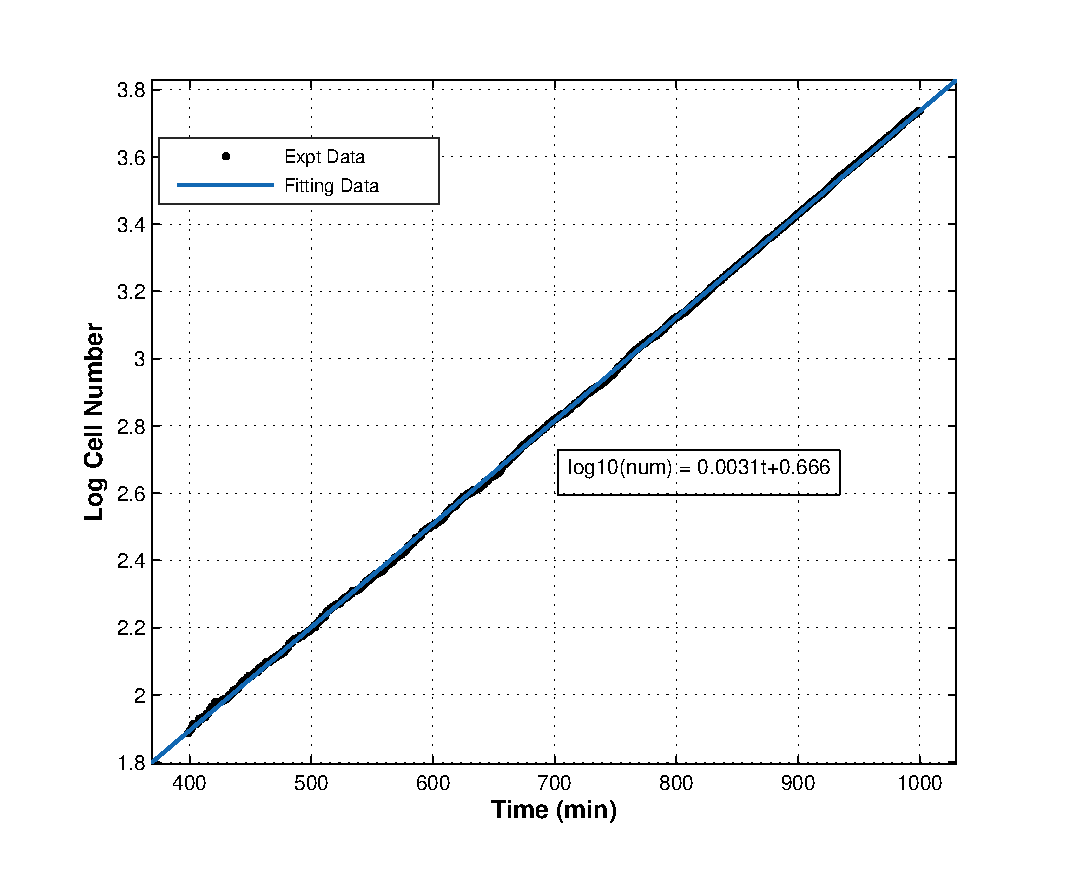
\includegraphics[scale=.8]{./figure/num_wt_fit.eps}
  \caption{The growth of a wild-type cell colony. The number of cells increases exponentially.}
  \label{fig:wt_fit}
\end{figure}



%================================================================================
%================================================================================
%================================================================================
\newpage
\section{Results of The Hybrid Model with Mutations on Raffinose}
\subsection{Results of The Deterministic Simulation}
Deterministic simulations are executed on the hybrid model with mutations on Raffinose. 
Results are shown in Table \ref{tab:raffinose}.
A mother cell can divide four times. To make mother cells viable on Raffinose, 
$k_{s,Clb2}$ is needed to be reduced from $0.45*k_{s,Clb2}$ to $0.43*k_{s,Clb2}$.
\begin{table}[H]
  \centering
  \caption{Deterministic simulation results of cells with mutations in Raffinose.}
  \vspace{0.2in}
  \begin{tabular}{|c|c|c|c|c|c|c|}
  \hline 
    \multirow{2}{*}{ } & 
    \multicolumn{2}{c|}{CLB2-db$\Delta$} & 
    \multicolumn{2}{c|}{clb5$\Delta$} & 
    \multicolumn{2}{c|}{CLB2-db$\Delta$clb5$\Delta$} \\
  \hline
    & Mother & Daughter & Mother & Daughter & Mother & Daughter \\
  \hline
  \hline
  Chen's Model  & Viable                 &  Viable  & Viable & Viable & Viable  & Viable \\
  Hybrid Model  & Viable in 4 divisions  &  Viable  & Viable & Viable & Viable in 4 divisions & Viable \\
  \hline
  \end{tabular}
  \label{tab:raffinose}
\end{table}

\subsection{Results of The Hybrid Method}
The hybrid method was executed on this hybrid cell cycle model with \textbf{double mutations} on Raffinose.
The probability a cell divides successfully is \textbf{0.667}. The cell number increment in a colony is 
plotted in Figure \ref{fig:rf_fit}.
\begin{figure}[H]
  \centering
  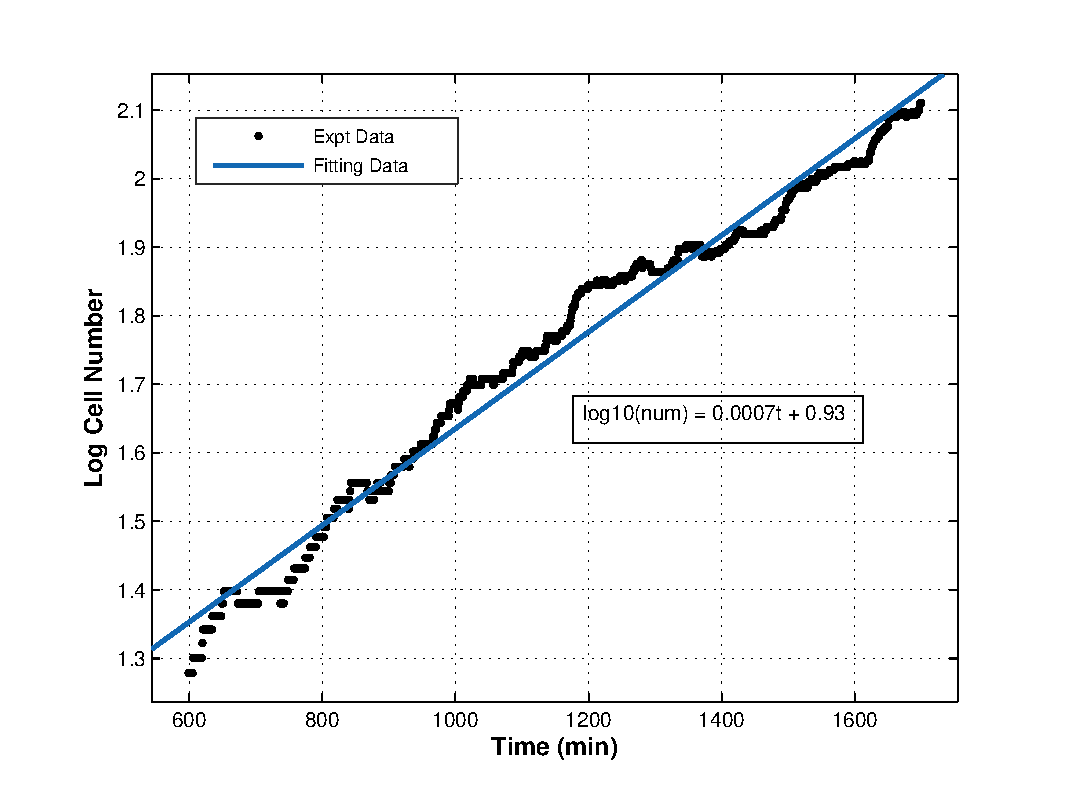
\includegraphics[scale=.8]{./figure/num_rf_fit.eps}
  \caption{The increment of cell numbers. Cells in the colony have double mutations and grow up in Raffinose.
  The number of cells increases exponentially.}
  \label{fig:rf_fit}
\end{figure}


\newpage
\section{Results of The Hybrid Model with Mutations on Glucose}
\subsection{Results of The Deterministic Simulation}
Deterministic simulations are executed on the hybrid model with mutations on Glucose. 
Results are shown in Table \ref{tab:glucose}.
\begin{table}[H]
  \centering
  \caption{Deterministic simulation results of cells with mutations on Glucose.}
  \vspace{0.2in}
  \begin{tabular}{|c|c|c|c|c|c|c|}
  \hline 
    \multirow{2}{*}{ } & 
    \multicolumn{2}{c|}{CLB2-db$\Delta$} & 
    \multicolumn{2}{c|}{clb5$\Delta$} & 
    \multicolumn{2}{c|}{CLB2-db$\Delta$clb5$\Delta$} \\
  \hline
    & Mother & Daughter & Mother & Daughter & Mother & Daughter \\
  \hline
  \hline
  Chen's Model  & Inviable  &  Inviable  & Viable & Viable & Inviable  & Inviable \\
  Hybrid Model  & Inviable  &  Inviable  & Viable & Viable & Inviable  & Inviable \\
  \hline
  \end{tabular}
  \label{tab:glucose}
\end{table}

\subsection{Results of The Hybrid Method}
The hybrid method was executed on this hybrid cell cycle model with \textbf{double mutations} on Glucose.
The probability a cell divides successfully is \textbf{0.213}. The cell number increment in a colony is 
plotted in Figure \ref{fig:gl_num}.
\begin{figure}[H]
  \centering
  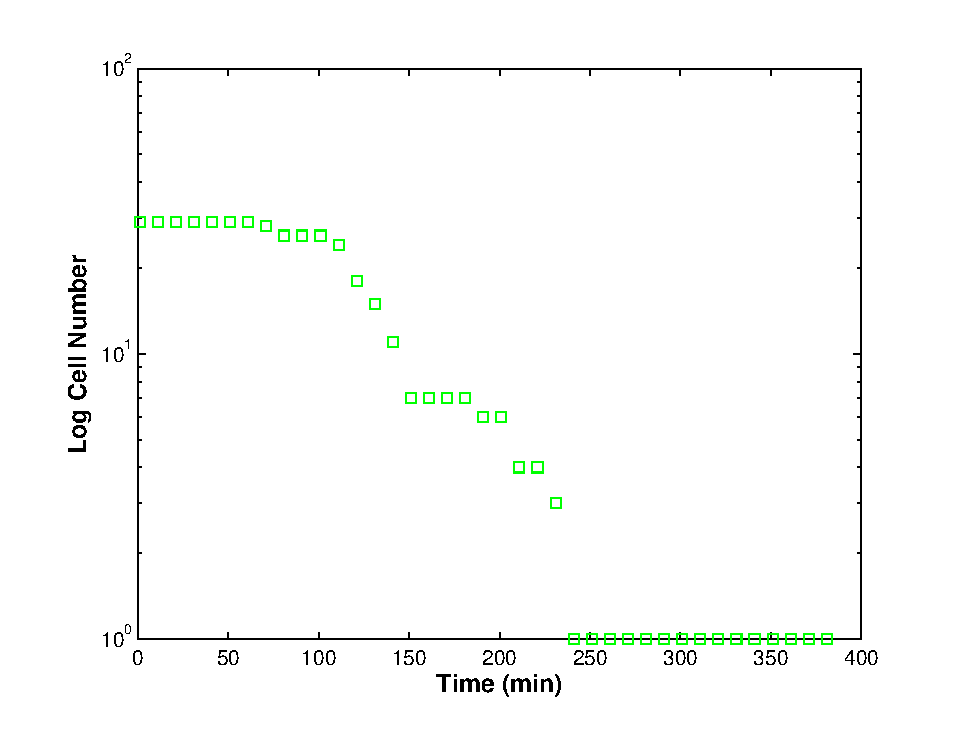
\includegraphics[scale=.7]{./figure/num_gl.eps}
  \caption{The increment of cell numbers. Cells in the colony have double mutations and grow up in Glucose.
  The colony vanishes under this condition.}
  \label{fig:gl_num}
\end{figure}


\begin{figure}[H]
  \centering
  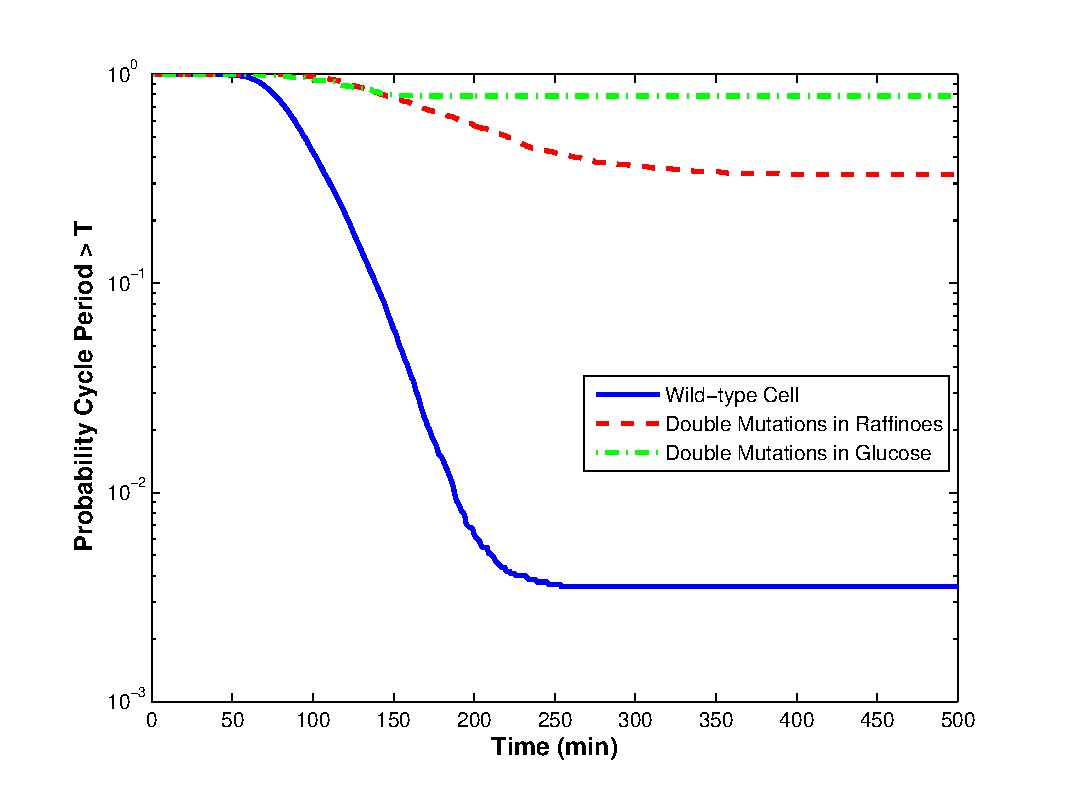
\includegraphics[scale=.7]{./figure/cycle_prob.eps}
  \caption{The probability that the cell cycle period is greater than a specified time for the three 
           simulation experiments.}
  \label{fig:cycle_prob}
\end{figure}


\newpage
\section{Results of The Hybrid Model with Mutations on Galactose}
\subsection{Results of The Deterministic Simulation}
Deterministic simulations are carried out on the hybrid model with mutations on Galactose. 
Results are shown in Table \ref{tab:galactose}.
A mother cell can divide only once with smaller cell size.
\begin{table}[H]
  \centering
  \caption{Deterministic simulation results of cells with mutations on Galactose.}
  \vspace{0.2in}
  \begin{tabular}{|c|c|c|c|c|c|c|}
  \hline 
    \multirow{2}{*}{ } & 
    \multicolumn{2}{c|}{CLB2-db$\Delta$} & 
    \multicolumn{2}{c|}{clb5$\Delta$} & 
    \multicolumn{2}{c|}{CLB2-db$\Delta$clb5$\Delta$} \\
  \hline
    & Mother & Daughter & Mother & Daughter & Mother & Daughter \\
  \hline
  \hline  
  Hybrid Model  & Viable in 1 division  &  Viable  & Viable & Viable & Viable in 1 division & Viable \\
  \hline
  \end{tabular}
  \label{tab:galactose}
\end{table}

\subsection{Results of The Hybrid Method}
The hybrid method was carried out on this hybrid cell cycle model with \textbf{double mutations} on Galactose.
The probability a cell divides successfully is \textbf{0.60}. The cell number increment in a colony is 
plotted in Figure \ref{fig:ga_fit}.
\begin{figure}[H]
  \centering
  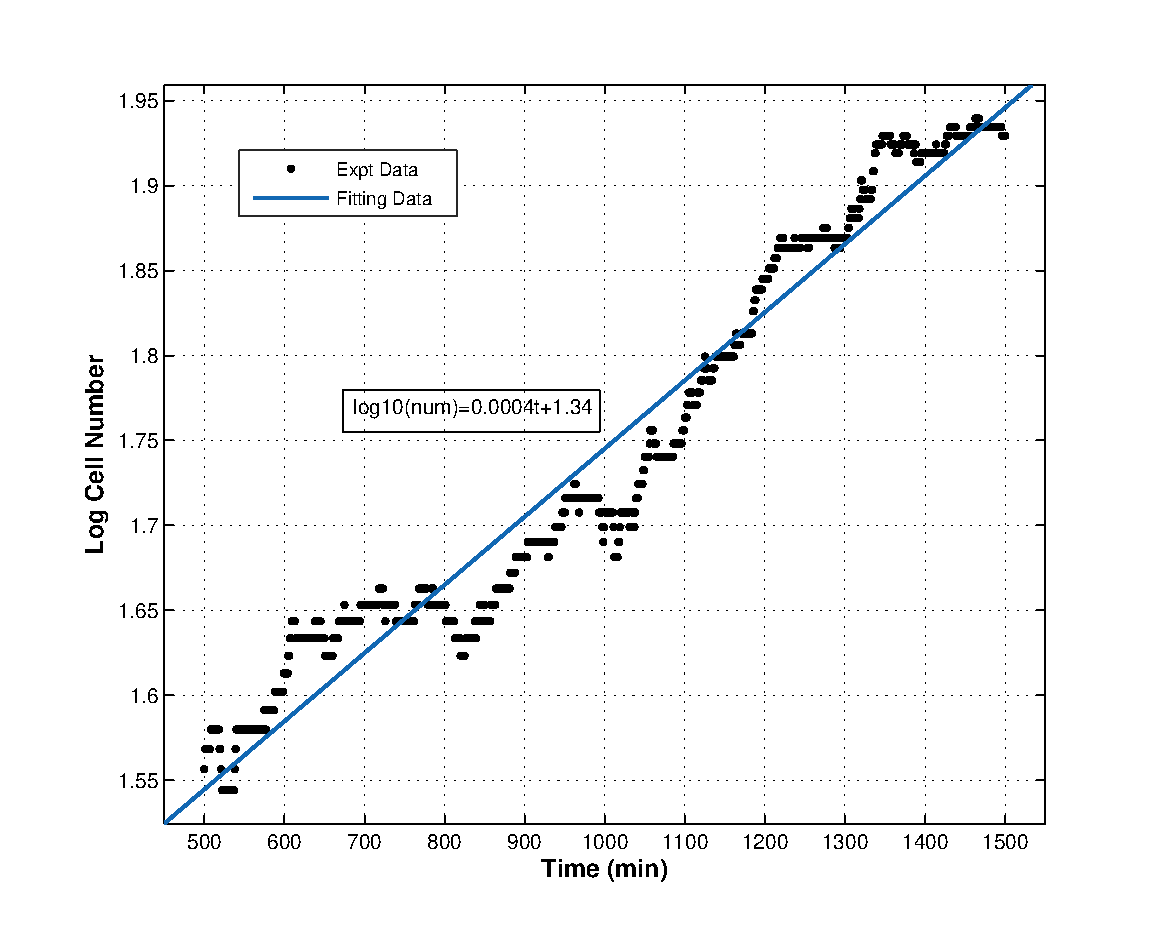
\includegraphics[scale=.8]{./figure/num_ga_fit.eps}
  \caption{The increment of cell numbers. Cells in the colony have double mutations and grow up on Galactose.
  The number of cells increases exponentially.}
  \label{fig:ga_fit}
\end{figure}


\end{document}

